\documentclass{scrartcl} % scrartcl of scrreprt
% Include all project wide packages here.
\usepackage{fullpage}
\usepackage{polyglossia}
\setmainlanguage{dutch}
\usepackage{csquotes}
\usepackage{graphicx}
\usepackage{epstopdf}
\usepackage{pdfpages}
\usepackage{caption}
\usepackage[list=true]{subcaption}
\usepackage{float}
%\usepackage{mathtools}
\usepackage{standalone}
\usepackage{import}
\usepackage{tocloft}
\usepackage{wrapfig}
\usepackage{authblk}
\usepackage{array}
\usepackage{booktabs}
\usepackage[toc,page,title,titletoc]{appendix}
\usepackage{xunicode}
\usepackage{amsmath}
\usepackage{fontspec}
\usepackage{unicode-math}
\usepackage[
    backend=bibtexu,
	texencoding=utf8,
bibencoding=utf8,
    style=ieee,
    sortlocale=nl_NL,
    language=auto
]{biblatex}
\usepackage{listings}
\newcommand{\includecode}[3][c]{\lstinputlisting[caption=#2, escapechar=, style=#1]{#3}}
\newcommand{\superscript}[1]{\ensuremath{^{\textrm{#1}}}}
\newcommand{\subscript}[1]{\ensuremath{_{\textrm{#1}}}}


\newcommand{\chapternumber}{\thechapter}
\renewcommand{\appendixname}{Bijlage}
\renewcommand{\appendixtocname}{Bijlagen}
\renewcommand{\appendixpagename}{Bijlagen}

\usepackage[hidelinks]{hyperref} %<--------ALTIJD ALS LAATSTE

\renewcommand{\familydefault}{\sfdefault}

\setmainfont[Ligatures=TeX]{Myriad Pro}
\setmathfont{Asana Math}
\setmonofont{Lucida Console}

\usepackage{titlesec, blindtext, color}
\definecolor{gray75}{gray}{0.75}
\newcommand{\hsp}{\hspace{20pt}}
\titleformat{\chapter}[hang]{\Huge\bfseries}{\chapternumber\hsp\textcolor{gray75}{|}\hsp}{0pt}{\Huge\bfseries}
\renewcommand{\familydefault}{\sfdefault}
\renewcommand{\arraystretch}{1.2}
\setlength\parindent{0pt}

%For code listings
\definecolor{black}{rgb}{0,0,0}
\definecolor{browntags}{rgb}{0.65,0.1,0.1}
\definecolor{bluestrings}{rgb}{0,0,1}
\definecolor{graycomments}{rgb}{0.4,0.4,0.4}
\definecolor{redkeywords}{rgb}{1,0,0}
\definecolor{bluekeywords}{rgb}{0.13,0.13,0.8}
\definecolor{greencomments}{rgb}{0,0.5,0}
\definecolor{redstrings}{rgb}{0.9,0,0}
\definecolor{purpleidentifiers}{rgb}{0.01,0,0.01}


\lstdefinestyle{csharp}{
language=[Sharp]C,
showspaces=false,
showtabs=false,
breaklines=true,
showstringspaces=false,
breakatwhitespace=true,
escapeinside={(*@}{@*)},
columns=fullflexible,
commentstyle=\color{greencomments},
keywordstyle=\color{bluekeywords}\bfseries,
stringstyle=\color{redstrings},
identifierstyle=\color{purpleidentifiers},
basicstyle=\ttfamily\small}

\lstdefinestyle{c}{
language=C,
showspaces=false,
showtabs=false,
breaklines=true,
showstringspaces=false,
breakatwhitespace=true,
escapeinside={(*@}{@*)},
columns=fullflexible,
commentstyle=\color{greencomments},
keywordstyle=\color{bluekeywords}\bfseries,
stringstyle=\color{bluestrings},
identifierstyle=\color{purpleidentifiers}
}

\lstdefinestyle{vhdl}{
language=VHDL,
showspaces=false,
showtabs=false,
breaklines=true,
showstringspaces=false,
breakatwhitespace=true,
escapeinside={(*@}{@*)},
columns=fullflexible,
commentstyle=\color{greencomments},
keywordstyle=\color{bluekeywords}\bfseries,
stringstyle=\color{redstrings},
identifierstyle=\color{purpleidentifiers}
}

\lstdefinestyle{xaml}{
language=XML,
showspaces=false,
showtabs=false,
breaklines=true,
showstringspaces=false,
breakatwhitespace=true,
escapeinside={(*@}{@*)},
columns=fullflexible,
commentstyle=\color{greencomments},
keywordstyle=\color{redkeywords},
stringstyle=\color{bluestrings},
tagstyle=\color{browntags},
morestring=[b]",
  morecomment=[s]{<?}{?>},
  morekeywords={xmlns,version,typex:AsyncRecords,x:Arguments,x:Boolean,x:Byte,x:Char,x:Class,x:ClassAttributes,x:ClassModifier,x:Code,x:ConnectionId,x:Decimal,x:Double,x:FactoryMethod,x:FieldModifier,x:Int16,x:Int32,x:Int64,x:Key,x:Members,x:Name,x:Object,x:Property,x:Shared,x:Single,x:String,x:Subclass,x:SynchronousMode,x:TimeSpan,x:TypeArguments,x:Uid,x:Uri,x:XData,Grid.Column,Grid.ColumnSpan,Click,ClipToBounds,Content,DropDownOpened,FontSize,Foreground,Header,Height,HorizontalAlignment,HorizontalContentAlignment,IsCancel,IsDefault,IsEnabled,IsSelected,Margin,MinHeight,MinWidth,Padding,SnapsToDevicePixels,Target,TextWrapping,Title,VerticalAlignment,VerticalContentAlignment,Width,WindowStartupLocation,Binding,Mode,OneWay,xmlns:x}
}

%defaults
\lstset{
basicstyle=\ttfamily\small,
extendedchars=false,
numbers=left,
numberstyle=\ttfamily\tiny,
stepnumber=1,
tabsize=4,
numbersep=5pt
}
\addbibresource{../../library/bibliography.bib}

\author{}
\title{EPO3: Eindrapport - Decoder}

\begin{document}
\chapter{Ontwerpspecificaties van de GPU}
\label{ch:spec}

\section {Functie van de GPU}
Een GPU is elektrische schakeling ontworpen om aan de hand van input data het geheugen te vormen en te wijzigen, zodat het maken van afbeeldingen voor een screen buffer snel genoeg gaat voor een vloeiende beeld op het beelscherm. De GPU die voor  dit project ontworpen en gefabriceerd wordt, zal dezelfde functie hebben als een algemene GPU, maar voor dit project zijn er bepaalde beperkingen voor de IC, die worden beschreven in de " Randvoorwaarden van de IC".
\\De GPU zal opgebouwd moeten worden volgens het blokschema in figuur~\ref{overzichtGPU} aan het einde van dit hoofdstuk.
Zoals er in het blokschema gezien kan worden, zijn er een aantal externe interacties nodig om met de GPU een afbeelding op een monitor te laten schrijven. Ten eerste is er een CPU nodig om de benodigde data voor een schermafbeelding van één frame te sturen naar de GPU. Daarna zal de GPU deze data moeten omzetten naar zijn pixel equivalent en deze op een screenbuffer in het externe SRAM moeten schrijven, zodat de frame niet wordt overgeschreven bij het invoeren van de volgende frame, die op de volgende screenbuffer wordt geschreven. Ook moet de GPU het huidige frame van de screenbuffer uit het SRAM kunnen uitlezen, om deze vervolgens te modificeren tot een signaal dat door een VGA monitor verwerkt kan worden tot een schermafbeelding. Deze externe SRAM is nodig, omdat er op de chip zelf niet genoeg transistoren zijn om een RAM te maken, die screenbuffers kan aanmaken,
%Aanpassen deze figuur
\begin{figure}[H]
\centering
        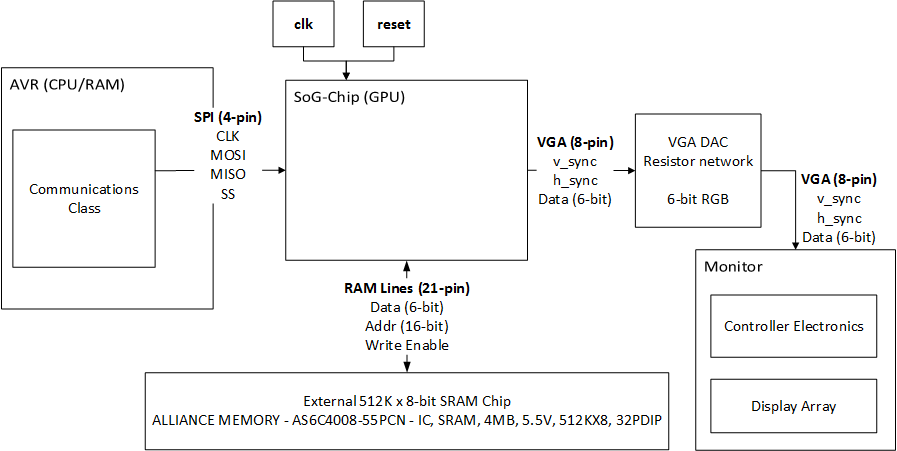
\includegraphics[scale=0.9]{Resource/system_overview.png}
        \caption{overzicht GPU}
        \label{fig:overzichtGPU}
\end{figure} 


\section {Functionele Eisen}
Om een GPU van acceptabel niveau te ontwerpen, zijn er deze funtionele eisen gesteld.
\begin {itemize}
\item De GPU moet aangestuurd worden door een CPU.
\item De GPU moet gebruik maken van externe RAM.
\item De GPU moet in staat zijn om een aantal elementaire vormen (pixels, vierkanten en lijnen) op een beeldscherm te tekenen.
\item De GPU krijgt data betreffende deze elementaire vormen vanuit de CPU (een AVR), bijvoorbeeld voor een vierkant bestaat de data uit de x- en y-coördinaten, breedte, hoogte en kleur.
\item De communicatie tussen de CPU en de GPU moet met een SPI verbinding gedaan worden.
\item Het beeldscherm wordt aangestuurd middels een VGA-signaal, die wordt gestuurd door de GPU.
\item De GPU moet minimaal 160x120 individuele beeldpunten kunnen tekenen met 6-bit RGB kleur mogelijkheden.
\item De communicatie tussen de externe SRAM en de GPU moet met een parralele bus verbinding tot stand gebracht worden.
\item het externe SRAM moet weten wanneer de GPU erop gaat schrijven. Daar is het Write Enable signaal uit figuur~\ref{overzichtGPU} voor.
\end{itemize}

\section {Randvoorwaarden van de IC}

Voor de te gebruiken IC zijn er een aantal randvoorwaarden waaraan gehouden moet worden wil dit project goed slagen. Deze randvoorwaarden zijn gegeven in de projecthandleiding\cite {epo3-manual}.

\begin {itemize}
\item  Voor de FSM’s (Finite State Machine) mogen alleen deze van het Moore-type gebruikt
worden.
\item Als de schakeling geactiveerd wordt, moeten alle FSM’s in hun resetoestand komen door middel van een resetsignaal.
\item Voor het genereren van het kloksignaal kan gebruik gemaakt worden van een kristal van 6.144 MHz of 32 kHz, dat extern wordt aangesloten aan de IC met 2 pinnen.
\item Het kristal voor de klok wordt met 2 pinnen aangesloten aan de IC en heeft een klokfrequentie is 6.144 Mhz.
\item Het streven is om zo weinig mogelijk componenten extern te gebruiken. De dissipatie van de chip dient echter ook beperkt te zijn. Dit geeft een compromis voor de maximale stroom
die de elektronica mag dissiperen voor de aansturing van de LEDs, etc.
\item De voedingsspanning van het IC bedraagt 5 Volt.
\item Het IC wordt gemaakt met een 1.6 µm nwell-CMOS proces(het Philips C3DM proces).
\item  Het beschikbare chip-oppervlak is circa $0.4  cm^2$ , hetgeen overeenkomt met ongeveer 40.000 transistorparen, die gelijk zijn verdeeld over 2 bond bars.
\item  Er zijn op het IC 36 verbonden aansluitingen, waarvan 4 pinnen voor de voeding zijn.
\end {itemize}

\textbf{Parameters Sea-of-Gates}
\begin {itemize}
\item $V_{DD} = 5V$
\item$ V_{T0} = 0.7V$
\item  $t_{ox} = 25 ∗ 10^{−9}m$
\item Nmos L×W = 1.6 × 23.2µm
\item Pmos L×W = 1.6 × 29.6µm
\end {itemize}


\end{document}
